%!TEX root = ../thesis.tex

\begin{figure}
\centering
\begin{subfigure}{.5\textwidth}
\centering
  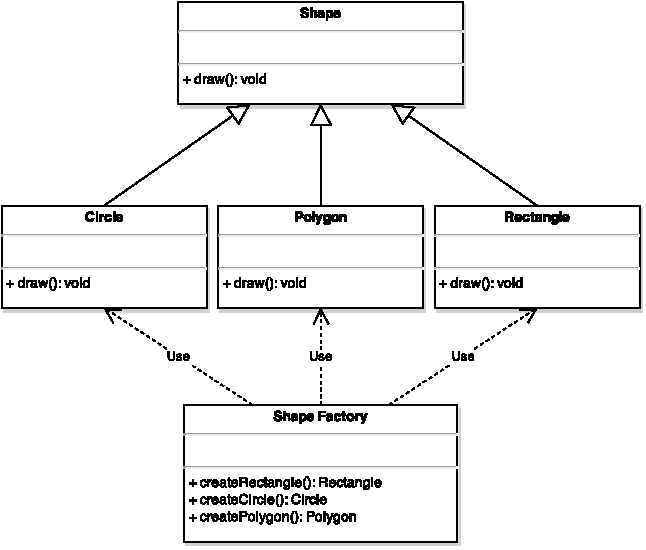
\includegraphics[width=.95\linewidth]{../images/code-visualisations/class-diagram.pdf}
  \caption{Class diagram}
  \label{fig:class-diagram}
\end{subfigure}%
\begin{subfigure}{.5\textwidth}
\centering
  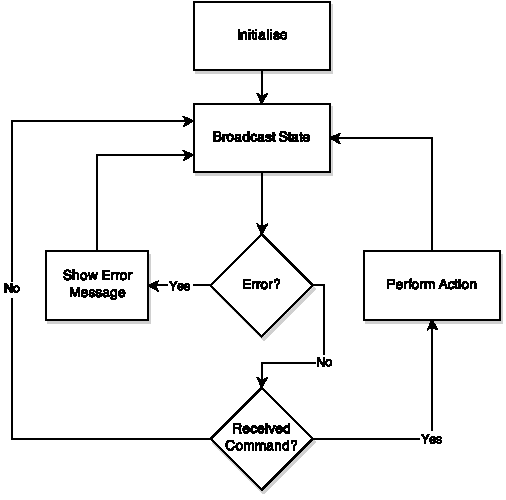
\includegraphics[width=.8\linewidth]{../images/code-visualisations/flow-chart.pdf}
  \caption{Flow chart}
  \label{fig:flow-chart}
\end{subfigure}\\
\vspace{5mm}

\begin{subfigure}{.5\textwidth}
\centering
  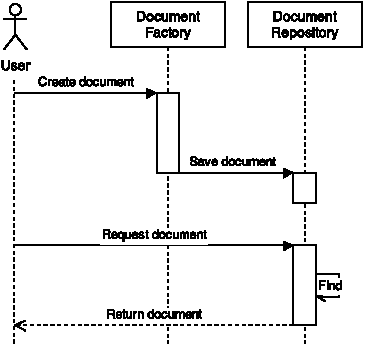
\includegraphics[width=.8\linewidth]{../images/code-visualisations/sequence-diagram.pdf}
  \caption{Sequence diagram}
  \label{fig:sequence-diagram}
\end{subfigure}%
\begin{subfigure}{.5\textwidth}
\centering
  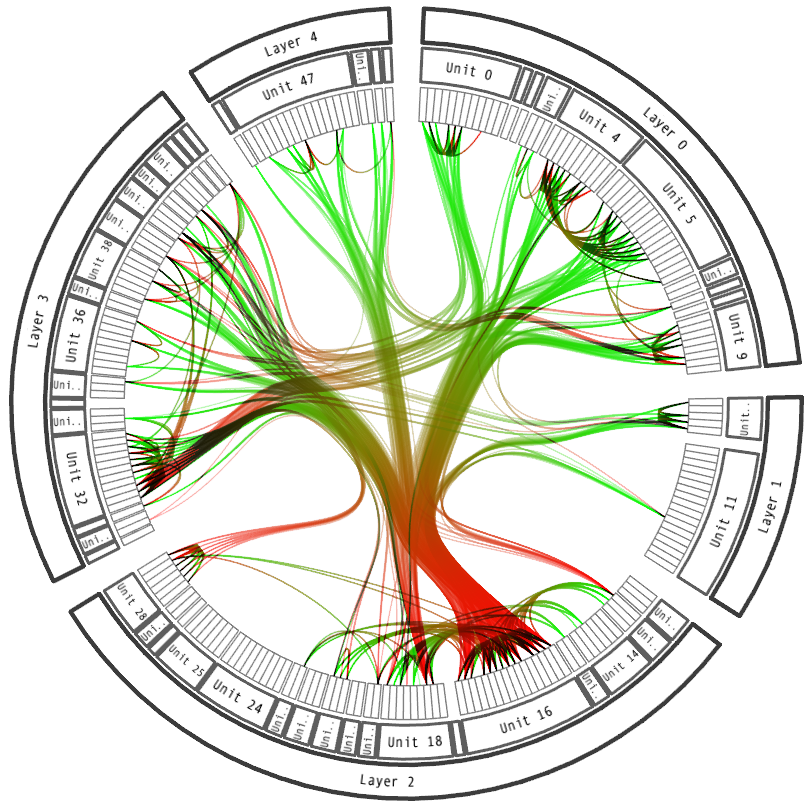
\includegraphics[width=0.8\linewidth]{../images/code-visualisations/bundle-graph.png}
  \caption{Edge bundled graph}
  \label{fig:bundle-graph}
\end{subfigure}

\caption[Existing software diagramming and graphing techniques]{Existing software diagramming and graphing techniques.}
\label{fig:code-diagrams}
\end{figure}